\documentclass[aspectratio=169,11pt,t]{beamer}
% ============================================================
%  ksa-cs-v2: ksa-cs-lecture-template.tex 스타일 + 한글, v2 덱(16:9)용.
%    - 짙은 네이비 헤드라인 (섹션 이름 + 프레임마다 점)
%    - 꽉 찬 파란 제목 막대, 둥근 그림자 블록
%    - 한글: Noto Sans CJK KR (fontspec)
%  사용:
%    \documentclass[aspectratio=169,11pt,t]{beamer}
%    \input{<..>/theme/ksa-cs-v2.tex}
%  ksa-theme.tex 의 매크로(\kb \kq, ksablue/ksared 등)도 같은 이름으로 둔다
%  -> v2 덱 본문을 거의 그대로 옮길 수 있다.
% ============================================================

\usepackage{fontspec}
\usepackage{amsmath,amssymb}
\usepackage{tikz}
\usepackage{listings}
\usepackage{graphicx}
\usepackage{booktabs}
\usepackage{varwidth}
% enumitem 은 넣지 않는다 (beamer 글머리표가 사라진다)

\defaultfontfeatures{Ligatures=TeX}
\setmainfont{Noto Sans CJK KR}
\setsansfont{Noto Sans CJK KR}
\setmonofont{Noto Sans Mono CJK KR}[Scale=0.92]
\usefonttheme{professionalfonts}

% ---------- 기본 틀 ----------
\usetheme{default}
\useinnertheme[shadow=true]{rounded}
\setbeamertemplate{navigation symbols}{}
\setbeamersize{text margin left=1em,text margin right=1em}

% ---------- 색 (템플릿 원본 값) ----------
\definecolor{navydark}{HTML}{191959}
\definecolor{navydim}{HTML}{8888B0}
\definecolor{navytitle}{HTML}{262686}
\definecolor{navyblue}{HTML}{3333B2}
\definecolor{blockbodybg}{HTML}{E9E9F3}
\definecolor{examplegreen}{HTML}{006000}
\definecolor{examplebg}{HTML}{E5EFE5}
\definecolor{alertred}{HTML}{BF0000}
\definecolor{alertbg}{HTML}{F9E5E5}
% ksa-theme.tex 와 같은 이름 (본문 호환)
\colorlet{ksablue}{navytitle}
\colorlet{ksabluedk}{navydark}
\definecolor{ksagold}{HTML}{D6CBB1}
\definecolor{ksagolddk}{HTML}{A9976B}
\colorlet{ksared}{alertred}
\definecolor{ksagray}{HTML}{5B5B5B}

\setbeamercolor{structure}{fg=navyblue}
\setbeamercolor{alerted text}{fg=alertred}
\setbeamercolor{frametitle}{bg=navytitle,fg=white}
\setbeamercolor{title}{fg=white,bg=navytitle}
\setbeamercolor{block title}{bg=navytitle,fg=white}
\setbeamercolor{block body}{bg=blockbodybg,fg=black}
\setbeamercolor{block title example}{bg=examplegreen,fg=white}
\setbeamercolor{block body example}{bg=examplebg,fg=black}
\setbeamercolor{block title alerted}{bg=alertred,fg=white}
\setbeamercolor{block body alerted}{bg=alertbg,fg=black}
\setbeamercolor{item}{fg=navyblue}
\setbeamertemplate{itemize item}[circle]
\setbeamertemplate{itemize subitem}[triangle]

% ---------- 헤드라인: miniframes (섹션 이름 + 점) ----------
\useoutertheme[subsection=false]{miniframes}
\setbeamerfont{section in head/foot}{size=\tiny}
\setbeamercolor{section in head/foot}{bg=navydark,fg=white}
\setbeamercolor{mini frame}{fg=white}
\setbeamertemplate{mini frames}[circle]

% ---------- 제목 막대: 폭 꽉 채움, 두 줄까지 ----------
\setbeamerfont{frametitle}{size=\normalsize,series=\bfseries}
\setbeamertemplate{frametitle}{%
  \nointerlineskip
  \begin{beamercolorbox}[wd=\paperwidth,ht=2.7ex,dp=1.1ex,leftskip=.3cm,rightskip=.3cm]{frametitle}%
    \usebeamerfont{frametitle}\insertframetitle
  \end{beamercolorbox}}

% ---------- 쪽 번호: 오른쪽 아래 ----------
\setbeamertemplate{footline}{%
  \hfill
  {\color{navydim}\scriptsize\insertframenumber\,/\,\inserttotalframenumber}%
  \hspace{3mm}\vspace{2mm}%
}

% ---------- 표지: 템플릿처럼 헤드라인은 그대로, 가운데 둥근 그림자 상자에 제목 한 줄 ----------
% 덱에서:  {\setbeamertemplate{footline}{}\begin{frame}[c,noframenumbering]\titlepage\end{frame}}
\setbeamercolor{title}{fg=white,bg=navyblue}
\makeatletter
\setbeamertemplate{title page}{%
  \vfill
  \centering
  \begin{minipage}{0.84\paperwidth}
  \begin{beamercolorbox}[wd=\linewidth,sep=7pt,center,rounded=true,shadow=true]{title}
    {\usebeamerfont{title}\inserttitle\par}%
    \ifx\insertsubtitle\@empty\else\vskip0.4em{\usebeamerfont{subtitle}\insertsubtitle\par}\fi
  \end{beamercolorbox}
  \end{minipage}\par\vskip1.6em
  {\usebeamerfont{author}\color{navytitle}\insertauthor\par}\vskip0.3em
  {\usebeamerfont{institute}\color{ksagray}\insertinstitute\par}
  \vfill
}
\makeatother
\setbeamerfont{title}{series=\bfseries,size=\Large}
\setbeamerfont{subtitle}{size=\normalsize}
\setbeamerfont{author}{size=\normalsize}
\setbeamerfont{institute}{size=\small}

% ksa-theme 호환: 덱이 \renewcommand{\ksacredit}{..} 를 해도 되게 (꼬리말에는 안 쓴다)
\newcommand{\ksacredit}{}

% ---------- 강조 ----------
\newcommand{\hl}[1]{\textcolor{alertred}{#1}}
\newcommand{\hlb}[1]{\textcolor{navyblue}{#1}}
\newcommand{\kb}[1]{\textbf{\color{ksablue}#1}}
\newcommand{\kq}[1]{\textbf{\color{ksared}#1}}

% ---------- 파이썬 코드 (템플릿과 같은 색) ----------
\definecolor{codekw}{HTML}{0033B3}
\definecolor{codebuiltin}{HTML}{BF0000}
\definecolor{codestr}{HTML}{067D17}
\definecolor{codecomment}{HTML}{8C8C8C}
\definecolor{codenum}{HTML}{1750EB}
\lstdefinestyle{py}{
  language=Python, basicstyle=\ttfamily\scriptsize,
  keywordstyle=\color{codekw}\bfseries, stringstyle=\color{codestr},
  commentstyle=\color{codecomment}\itshape, numberstyle=\color{codenum},
  emph={print,len,range,sum,input,int,str,float,list,dict,append,remove,sorted,abs,min,max},
  emphstyle=\color{codebuiltin}, showstringspaces=false, keepspaces=true,
  columns=fixed, basewidth=0.52em, aboveskip=1mm, belowskip=1mm, xleftmargin=2mm,
  breaklines=true
}
\lstset{style=py}

% 원본 덱 (ksa-theme): slides/v2/ml1/week02/precision_recall/ -- 그림은 거기 figs/ 를 그대로 쓴다
\setbeamerfont{author}{size=\normalsize}
\setbeamerfont{institute}{size=\small}
\graphicspath{{../../../v2/ml1/week02/precision_recall/figs/}{../../../assets/}}
\makeatletter
\newcommand{\markpage}[1]{\protected@write\@auxout{}{\string\newlabel{#1}{{\the\c@framenumber}{}}}\hypertarget{#1}{}}
\newcommand{\pref}[1]{\hyperlink{#1}{\textcolor{ksagolddk}{(p.\ref{#1})}}}
\makeatother

\renewcommand{\ksacredit}{Machine Learning and Deep Learning \,\textperiodcentered\, 정밀도와 재현율}
\title{정밀도와 재현율 (Precision \& Recall)}
\subtitle{정확도 90\%의 함정}
\author{Machine Learning and Deep Learning}
\institute{한국과학영재학교 (KSA)}
\date{}
\begin{document}
{\setbeamertemplate{footline}{}\begin{frame}[c,noframenumbering]\titlepage\end{frame}}

\section{질문}
% --- 오늘의 질문
\begin{frame}{오늘의 질문}
\vfill
\begin{columns}[c]
\begin{column}{0.4\textwidth}\centering
\includegraphics[width=0.9\linewidth]{pr_hook.png}\end{column}
\begin{column}{0.56\textwidth}\centering
{\Large 학교 100명 중 독감 \textcolor{ksared}{10명}}\\[1em]
{\large 모두 ``건강''이라고 찍는 AI}\\[0.4em]
{\Large 정확도 = \kq{90\%}}\\[1em]
{\large 좋은 AI일까?}
\end{column}
\end{columns}
\vfill
\note{학교 학생 100명 중 독감에 걸린 학생은 빨간 10명입니다. 여기에 아무것도 보지 않고 모든 학생을 건강하다고 찍는 AI가 있습니다. 이 AI의 정확도는 몇 퍼센트일까요? 건강한 90명은 그냥 맞히니까 90퍼센트입니다. 숫자만 보면 꽤 좋아 보이는데, 정말 좋은 AI일까요?}
\end{frame}

\section{정확도}
% --- 정확도
\begin{frame}{정확도: 맞힌 수 $\div$ 전체}
\vfill
\centering
{\LARGE\[ \text{accuracy} = \frac{\text{맞힌 수}}{\text{전체}} = \frac{90}{100} = 90\% \]}\vskip0.6em
{\large 건강한 90명은 그냥 맞힌다 \qquad 찾아낸 독감 학생은 \kq{0명}}\\[0.8em]
{\small 한쪽이 훨씬 많은 데이터 (쏠린 데이터, imbalanced) 에서는 정확도가 속인다}
\vfill
\note{정확도는 맞힌 수를 전체로 나눈 겁니다. 건강한 90명을 건강하다고 했으니 90명 맞혔고, 90퍼센트입니다. 그런데 이 AI가 찾아낸 독감 학생은 0명입니다. 우리가 이 AI를 만든 이유는 독감 학생을 찾기 위해서였죠. 이렇게 한쪽이 훨씬 많은 데이터를 쏠린 데이터라고 하는데, 쏠린 데이터에서는 정확도가 속입니다. 스팸, 사기 거래, 희귀병처럼 우리가 찾고 싶은 것은 대부분 드뭅니다.}
\end{frame}

% --- 진짜 AI
\begin{frame}{진짜로 진단하는 AI}
\markpage{venn}
\vfill
\centering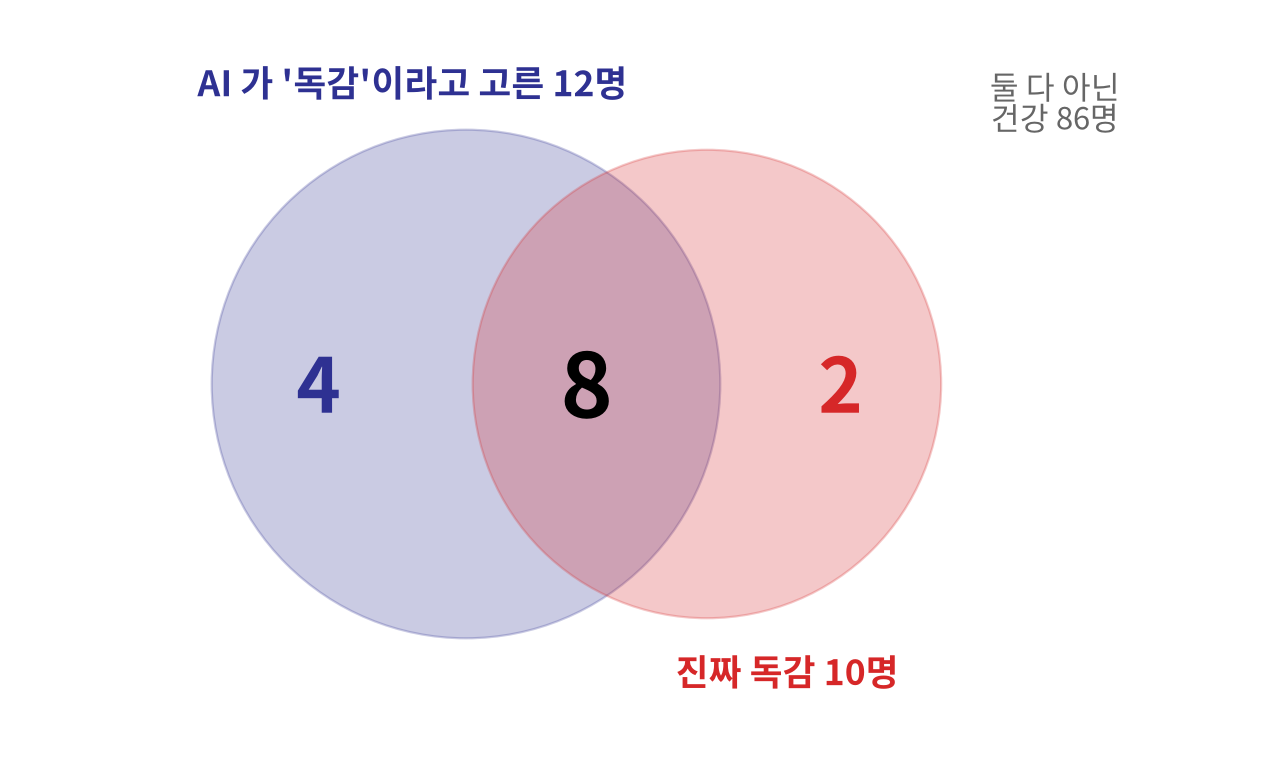
\includegraphics[width=0.56\linewidth]{pr_venn.png}\par\vskip0.2em
{\large AI 가 \textcolor{ksablue}{12명}을 ``독감''이라고 골랐다 \quad 진짜 독감 \textcolor{ksared}{10명}과 겹치는 건 \textbf{8명}}
\vfill
\note{이번에는 학생을 실제로 진찰해서 점수를 매기는 AI입니다. 이 AI는 12명을 독감이라고 골랐습니다. 파란 원입니다. 빨간 원은 진짜 독감에 걸린 10명입니다. 두 원이 겹치는 8명은 AI가 독감이라고 했고 실제로도 독감인 학생입니다. 파란 원에만 있는 4명은 건강한데 독감이라고 잘못 고른 학생, 빨간 원에만 있는 2명은 독감인데 AI가 놓친 학생입니다. 둘 다 아닌 86명은 건강하고 건강하다고 맞힌 학생입니다.}
\end{frame}

\section{혼동 행렬}
% --- 혼동 행렬
\begin{frame}{네 칸으로 정리: 혼동 행렬}
\markpage{cm}
\vfill
\centering
\renewcommand{\arraystretch}{1.5}
{\Large\begin{tabular}{r|c|c|}
\multicolumn{1}{r}{} & \multicolumn{1}{c}{실제 독감} & \multicolumn{1}{c}{실제 건강}\\\cline{2-3}
AI ``독감'' & \textbf{TP 8} & \textcolor{ksablue}{FP 4}\\\cline{2-3}
AI ``건강'' & \textcolor{ksared}{FN 2} & TN 86\\\cline{2-3}
\end{tabular}}\vskip0.8em
\renewcommand{\arraystretch}{1.2}
{\small\begin{tabular}{lll}
TP & true positive & 독감이라고 했고, 맞았다\\
FP & false positive & 독감이라고 했는데, 틀렸다 (헛짚음)\\
FN & false negative & 건강이라고 했는데, 틀렸다 (놓침)\\
TN & true negative & 건강이라고 했고, 맞았다
\end{tabular}}
\vfill
\note{앞의 두 원을 네 칸 표로 옮긴 것이 혼동 행렬, confusion matrix입니다. 가로는 실제, 세로는 AI의 판정입니다. 이름은 두 단어로 읽습니다. 뒤 단어 positive, negative는 AI가 뭐라고 했는지, 앞 단어 true, false는 그게 맞았는지입니다. TP 8명은 독감이라고 했고 맞았고, FP 4명은 독감이라고 했는데 틀린 헛짚음, FN 2명은 건강이라고 했는데 틀린 놓침, TN 86명은 건강이라고 했고 맞았습니다. 정확도는 맞은 칸 TP와 TN을 더해서 100으로 나눈 94퍼센트입니다.}
\end{frame}

% --- 정밀도
\begin{frame}{정밀도: AI 말이 맞았나?}
\markpage{prec}
\vfill
\centering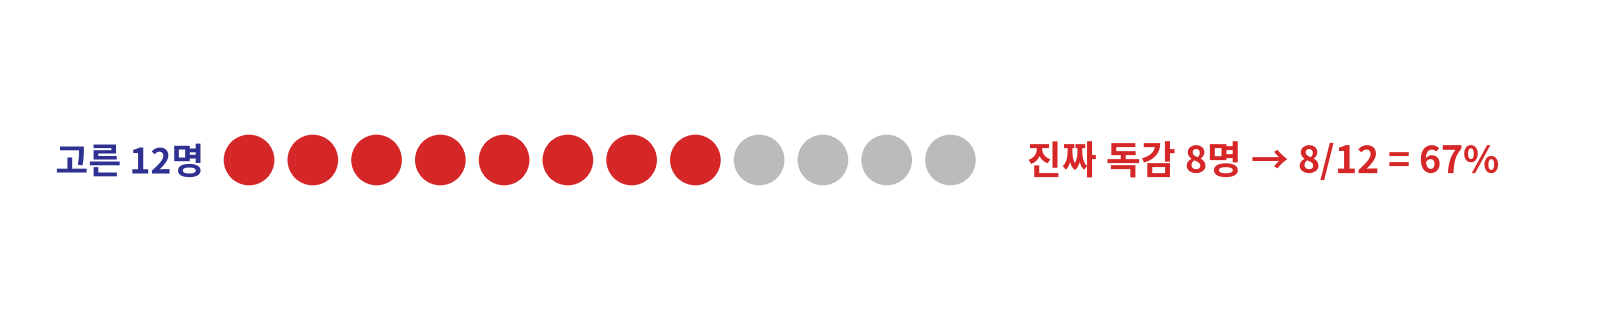
\includegraphics[width=0.8\linewidth]{pr_prec.png}\par\vskip0.3em
{\LARGE\[ \text{precision} = \frac{TP}{TP + FP} = \frac{8}{\underbrace{8 + 4}_{\text{AI 가 고른 12명}}} = 67\% \]}
{\large AI 가 ``독감''이라고 한 학생 중 진짜 독감의 비율}
\vfill
\note{첫 번째 지표는 정밀도입니다. AI가 독감이라고 고른 12명을 줄 세우면, 진짜 독감은 8명이고 4명은 헛짚었습니다. 8 나누기 12, 67퍼센트입니다. 분모가 AI가 고른 학생이라는 점이 중요합니다. 정밀도는 AI가 독감이라고 말했을 때 그 말이 얼마나 믿을 만한지, AI 말이 맞았나를 묻습니다.}
\end{frame}

% --- 재현율
\begin{frame}{재현율: 놓치지 않았나?}
\markpage{rec}
\vfill
\centering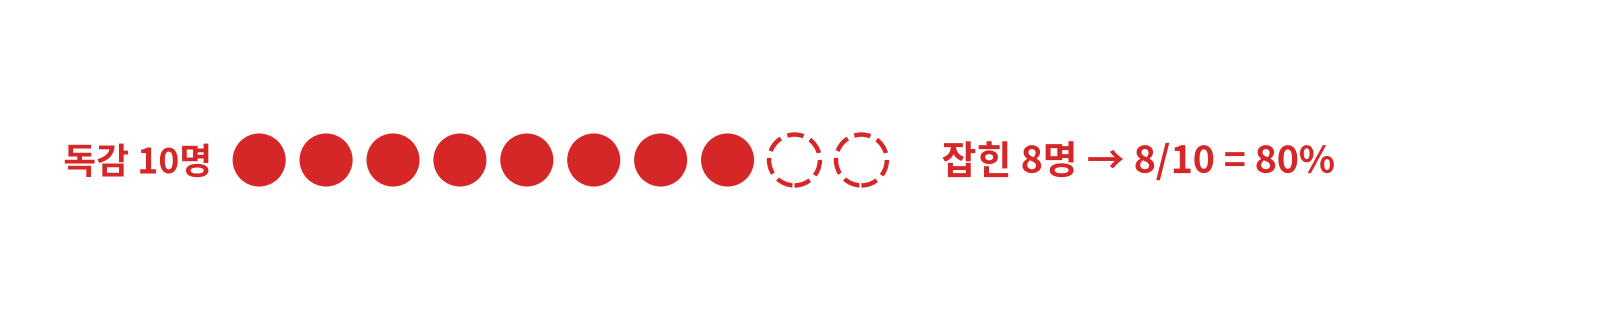
\includegraphics[width=0.8\linewidth]{pr_rec.png}\par\vskip0.3em
{\LARGE\[ \text{recall} = \frac{TP}{TP + FN} = \frac{8}{\underbrace{8 + 2}_{\text{진짜 독감 10명}}} = 80\% \]}
{\large 진짜 독감 학생 중 AI 가 찾아낸 비율 \qquad recall = 기억해 내기, 불러내기}
\vfill
\note{두 번째 지표는 재현율입니다. 이번에는 진짜 독감 학생 10명을 불러 모읍니다. AI가 잡아낸 건 8명이고 2명은 놓쳤습니다. 8 나누기 10, 80퍼센트입니다. 이번에는 분모가 진짜 독감 학생입니다. 재현율은 찾아야 할 것 중 얼마나 찾았는지, 놓치지 않았나를 묻습니다. 영어 recall은 원래 기억해 낸다, 불러낸다는 뜻입니다. 찾아야 할 것 중 얼마나 불러냈나로 기억하면 됩니다.}
\end{frame}

% --- 같은 분자 다른 분모
\begin{frame}{위는 같고, 아래만 다르다}
\vfill
\centering
{\LARGE\[ \text{precision} = \frac{TP}{\underbrace{TP + FP}_{\text{AI 가 고른 쪽}}} \qquad\qquad \text{recall} = \frac{TP}{\underbrace{TP + FN}_{\text{진짜인 쪽}}} \]}\vskip0.8em
\renewcommand{\arraystretch}{1.3}
{\large\begin{tabular}{lll}
정밀도 & 기준 = AI 의 판정 & 헛짚음(FP)이 많으면 떨어진다\\
재현율 & 기준 = 실제 정답 & 놓침(FN)이 많으면 떨어진다
\end{tabular}}\vskip0.6em
{\small 두 원 그림 \pref{venn}: 정밀도는 파란 원 안에서, 재현율은 빨간 원 안에서 겹친 부분의 비율}
\vfill
\note{두 식을 나란히 놓으면 분자는 둘 다 TP 8로 같고, 분모만 다릅니다. 정밀도는 AI가 고른 쪽, 파란 원을 기준으로 하고, 재현율은 진짜인 쪽, 빨간 원을 기준으로 합니다. 그래서 헛짚음 FP가 많으면 정밀도가 떨어지고, 놓침 FN이 많으면 재현율이 떨어집니다. 앞의 두 원 그림으로 말하면, 겹친 8명이 파란 원의 몇 퍼센트인가가 정밀도, 빨간 원의 몇 퍼센트인가가 재현율입니다.}
\end{frame}

% --- 모두 독감
\begin{frame}{모두 ``독감''이라고 찍으면?}
\vfill
\centering
{\Large\begin{tabular}{lccc}
 & 정확도 & 정밀도 & 재현율\\\hline\\[-0.8em]
모두 ``건강'' & 90\% & -- & \kq{0\%}\\[0.3em]
모두 ``독감'' & 10\% & \kq{10\%} & 100\%\\[0.3em]
진짜 AI & 94\% & 67\% & 80\%
\end{tabular}}\vskip1.0em
{\large 재현율 하나만 보면 \kq{``모두 독감''이 100\%}로 1등 \quad $\to$ 정밀도와 \kb{같이 봐야} 한다}
\vfill
\note{그러면 재현율만 높이면 될까요? 모든 학생을 독감이라고 찍으면 독감 10명을 하나도 놓치지 않으니 재현율 100퍼센트입니다. 대신 100명을 골라서 진짜는 10명이니 정밀도는 10퍼센트입니다. 반대로 모두 건강이라고 찍으면 정확도 90퍼센트지만 재현율 0퍼센트이고, 아무도 고르지 않았으니 정밀도는 계산할 수 없습니다. 한 지표만 보면 이렇게 찍는 AI가 1등이 될 수 있습니다. 그래서 정밀도와 재현율은 항상 같이 봅니다.}
\end{frame}

\section{F1}
% --- F1
\begin{frame}{둘을 숫자 하나로: F1 점수}
\vfill
\centering
{\LARGE\[ F_1 = \frac{2 \cdot \text{precision} \cdot \text{recall}}{\text{precision} + \text{recall}} \]}\vskip0.4em
{\large 진짜 AI: \; $\dfrac{2 \cdot 0.67 \cdot 0.80}{0.67 + 0.80} = 73\%$ \qquad 모두 ``독감'': \; $\dfrac{2 \cdot 0.10 \cdot 1.00}{0.10 + 1.00} = \kq{18\%}$}\\[0.8em]
{\small 조화평균: 둘 중 \kb{작은 쪽}에 끌려간다 \quad (그냥 평균이면 모두 ``독감''도 $\frac{10 + 100}{2} = 55\%$)}
\vfill
\note{두 숫자를 하나로 합치고 싶을 때 F1 점수를 씁니다. 그냥 평균이 아니라 조화평균입니다. 진짜 AI는 0.67과 0.8로 73퍼센트입니다. 모두 독감이라고 찍는 AI는 0.1과 1로 18퍼센트밖에 안 됩니다. 그냥 평균을 냈다면 55퍼센트로 꽤 좋아 보였을 겁니다. 조화평균은 둘 중 작은 쪽에 끌려가기 때문에, 한쪽만 높이는 꼼수를 막아 줍니다.}
\end{frame}

\section{기준선}
% --- 점수와 기준
\begin{frame}{AI 는 점수를 내고, 기준선이 판정한다}
\markpage{scores}
\vfill
\centering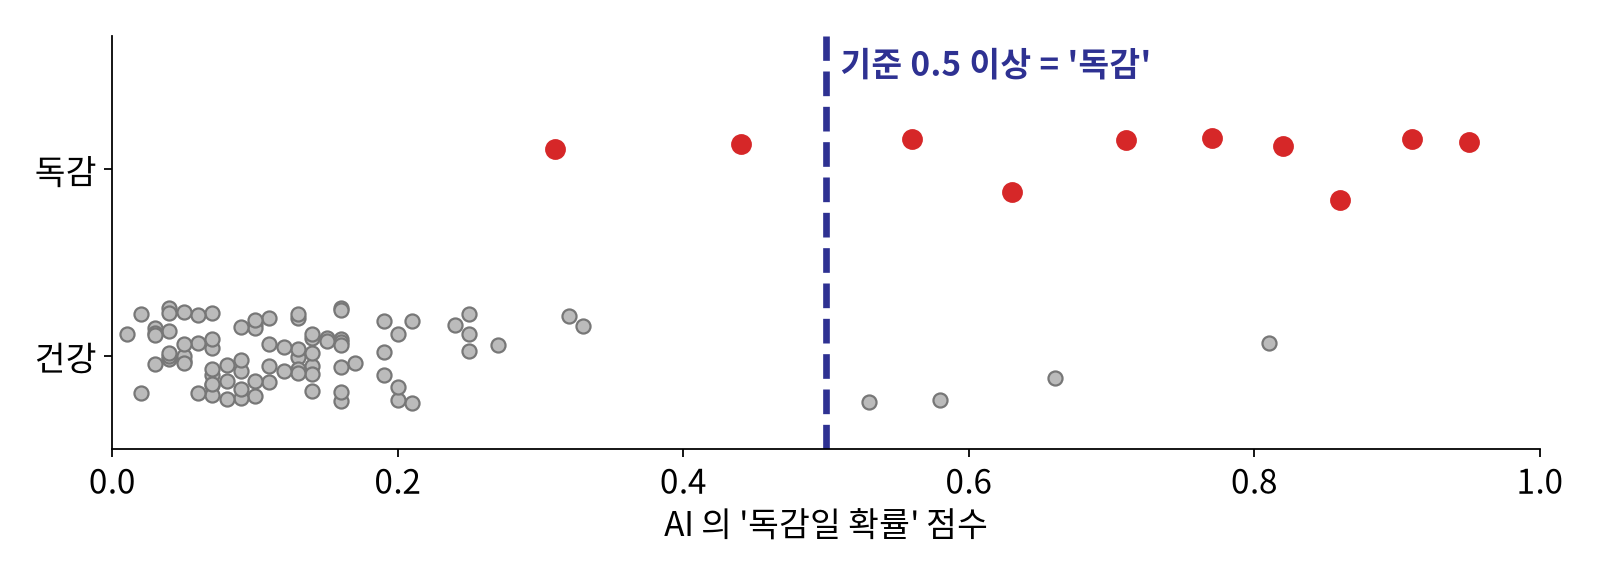
\includegraphics[width=0.82\linewidth]{pr_scores.png}\par\vskip0.2em
{\large 기준 오른쪽: \textcolor{ksared}{빨강 8} = TP, \; 회색 4 = FP \qquad 왼쪽: 빨강 2 = FN}
\vfill
\note{2주차 로지스틱회귀처럼, AI는 학생마다 독감일 확률 점수를 냅니다. 빨간 점이 독감 10명, 회색 점이 건강 90명의 점수입니다. 기준선 0.5보다 오른쪽이면 독감이라고 판정합니다. 기준선 오른쪽의 빨간 점 8개가 TP, 회색 점 4개가 FP, 왼쪽에 남은 빨간 점 2개가 FN입니다. 앞의 혼동 행렬은 이 그림에서 기준선을 0.5에 그었을 때의 결과입니다.}
\end{frame}

% --- 기준을 움직이면
\begin{frame}{기준선을 움직이면}
\vfill
\begin{columns}[c]
\begin{column}{0.56\textwidth}\centering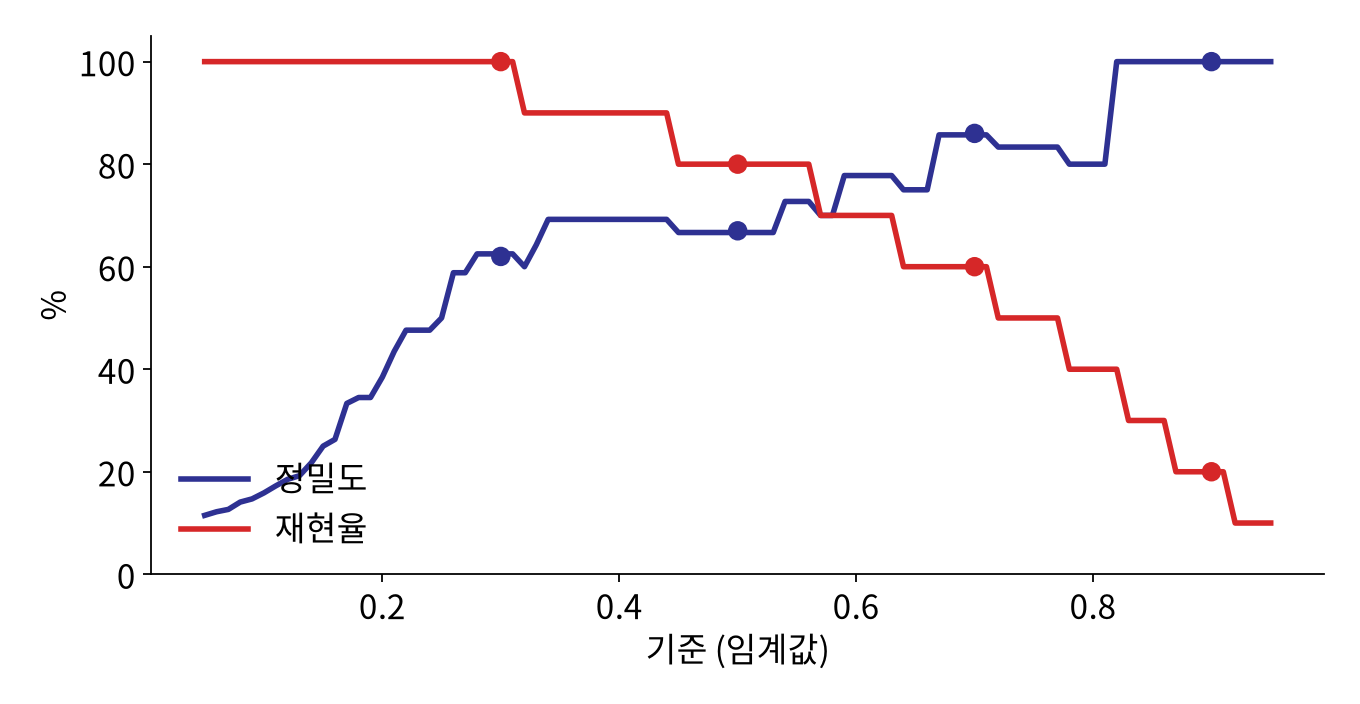
\includegraphics[width=\linewidth]{pr_threshold.png}\end{column}
\begin{column}{0.4\textwidth}
\renewcommand{\arraystretch}{1.3}
{\large\begin{tabular}{ccc}
기준 & 정밀도 & 재현율\\\hline
0.3 & 62\% & 100\%\\
0.5 & 67\% & 80\%\\
0.7 & 86\% & 60\%\\
0.9 & 100\% & 20\%
\end{tabular}}\vskip0.8em
{\large 올리면 \kb{정밀도} $\uparrow$ \kq{재현율} $\downarrow$}
\end{column}
\end{columns}
\vfill
\note{기준선을 움직여 봅니다. 0.9까지 올리면 정말 확실한 2명만 독감이라고 해서 정밀도는 100퍼센트지만 재현율은 20퍼센트입니다. 0.3까지 내리면 독감 10명을 모두 잡아서 재현율 100퍼센트지만 헛짚음이 6명이라 정밀도는 62퍼센트입니다. 기준을 올리면 정밀도가 오르고 재현율이 내려가는 줄다리기입니다. 그림의 선은 기준을 0.05부터 0.95까지 조금씩 움직인 결과입니다.}
\end{frame}

% --- 어디에 맞출까
\begin{frame}{무엇을 놓치면 더 곤란한가}
\vfill
\centering
\renewcommand{\arraystretch}{1.5}
{\large\begin{tabular}{lll}
\kq{재현율} 우선 & 암 검진, 공항 보안 검색 & 놓치면(FN) 위험 $\to$ 기준을 낮춘다\\
\kb{정밀도} 우선 & 스팸 필터, 유튜브 추천 & 헛짚으면(FP) 곤란 $\to$ 기준을 높인다
\end{tabular}}\vskip1.0em
{\large 기준선은 수학이 아니라 \textbf{문제}가 정한다}
\vfill
\note{그러면 기준은 어디에 둘까요. 정답은 문제에 따라 다릅니다. 암 검진이나 공항 보안 검색은 놓치는 게 훨씬 위험합니다. 헛짚으면 한 번 더 검사하면 되지만 놓치면 큰일이니까 기준을 낮춰 재현율을 높입니다. 반대로 스팸 필터는 중요한 정상 메일을 스팸함에 버리는 헛짚음이 더 곤란합니다. 스팸 몇 통 놓치는 건 참을 만하니 기준을 높여 정밀도를 높입니다. 기준선은 수학이 아니라 문제가 정합니다.}
\end{frame}

\section{연습}
% --- 문제풀이
\begin{frame}{문제풀이}
\vfill
\begin{enumerate}
\item 메일 1000통 중 스팸 50통. 필터가 60통을 스팸이라고 했고 그중 진짜 스팸은 45통. \; (a) TP, FP, FN, TN 은? \; (b) 정확도 · 정밀도 · 재현율은?\vskip0.8em
\item 정밀도 50\%, 재현율 100\% 인 모델의 F1 은? 그냥 평균과 비교하면?\vskip0.8em
\item 기준을 0.5 에서 0.7 로 올렸다. TP, FP, FN 중 늘어날 수 있는 것은?\vskip0.8em
\item 화재 경보기는 정밀도와 재현율 중 무엇을 우선해야 할까? 이유는?
\end{enumerate}
\vfill
\note{1번 답. TP는 45, 스팸이라고 한 60통 중 나머지 15통이 FP, 스팸 50통 중 못 잡은 5통이 FN, 남은 935통이 TN입니다. 정확도는 45 더하기 935를 1000으로 나눈 98퍼센트, 정밀도는 45 나누기 60으로 75퍼센트, 재현율은 45 나누기 50으로 90퍼센트입니다. 2번 답. 2 곱하기 0.5 곱하기 1을 1.5로 나눈 0.667, 약 67퍼센트이고, 그냥 평균 75퍼센트보다 작습니다. 3번 답. 기준을 올리면 독감이라고 하는 학생이 줄어드니 TP와 FP는 줄거나 그대로이고, 놓치는 FN만 늘어날 수 있습니다. 4번 답. 불이 났는데 안 울리는 놓침이 훨씬 위험하니 재현율입니다.}
\end{frame}

% --- 실습
\begin{frame}{실습}
\vfill
\centering\begin{tabular}{rl}
\large 1 & 슬라이드의 점수 100개로 혼동 행렬 · 정밀도 · 재현율 · F1 구현 $\to$ 8 / 4 / 2 / 86 재현\\[0.5em]
\large 2 & 기준을 0.05 $\sim$ 0.95 로 움직이며 정밀도 · 재현율 줄다리기 그리기\\[0.5em]
\large 3 & 실제 데이터: 피마 인디언 당뇨병 768명, 로지스틱회귀 + 기준 고르기
\end{tabular}\vskip1em
Pima Indians Diabetes (NIDDK; UCI) \\[0.4em]\href{https://colab.research.google.com/github/SuminHan/book-ml/blob/main/slides/v2/ml1/week02/precision_recall/lab/precision_recall.ipynb}{\textcolor{ksagolddk}{▶ Colab에서 실습 노트북 열기}}
\vfill
\note{실습은 세 부분입니다. 첫째, 슬라이드의 점수 100개로 혼동 행렬과 정밀도, 재현율, F1을 직접 구현해서 8, 4, 2, 86을 재현합니다. 둘째, 기준을 움직이며 정밀도와 재현율의 줄다리기를 그립니다. 셋째, 실제 의료 데이터인 피마 인디언 당뇨병 데이터 768명으로 로지스틱회귀를 학습하고, 재현율 80퍼센트를 넘기는 기준을 직접 고릅니다.}
\end{frame}

\section{정리}
% --- 정리
\begin{frame}{정리}
\vfill
\centering\large\begin{tabular}{l}
쏠린 데이터에서 \textbf{정확도}는 속인다 \quad (모두 ``건강'' $\to$ 90\%)\\[0.5em]
\kb{정밀도} $= TP / (TP + FP)$ \quad AI 말이 맞았나?\\[0.5em]
\kq{재현율} $= TP / (TP + FN)$ \quad 놓치지 않았나?\\[0.5em]
\textbf{F1} = 조화평균 \quad 기준선을 올리면 정밀도 $\uparrow$ 재현율 $\downarrow$
\end{tabular}
\vfill
\note{정리합니다. 쏠린 데이터에서 정확도는 속입니다. 모두 건강이라고 찍어도 90퍼센트가 나오니까요. 정밀도는 AI가 고른 것 중 진짜의 비율로, AI 말이 맞았나를 묻습니다. 재현율은 진짜 중 찾아낸 비율로, 놓치지 않았나를 묻습니다. 둘은 같이 봐야 하고, 하나로 합칠 때는 조화평균인 F1을 씁니다. 기준선을 올리면 정밀도가 오르고 재현율이 내려가니, 무엇을 놓치면 더 곤란한지로 기준을 정합니다. 다음 시간에는 기준선을 처음부터 끝까지 움직인 곡선 전체를 숫자 하나로 평가하는 PR-AUC를 배웁니다.}
\end{frame}
\end{document}
